\documentclass[a4paper]{report}
% Some basic packages
\usepackage[utf8]{inputenc}
\usepackage[T1]{fontenc}
\usepackage{textcomp}
\usepackage[english]{babel}
\usepackage{url}
\usepackage{graphicx}
\usepackage{float}
\usepackage{booktabs}
\usepackage{enumitem}

\pdfminorversion=7

% Don't indent paragraphs, leave some space between them
\usepackage{parskip}

% Hide page number when page is empty
\usepackage{emptypage}
\usepackage{subcaption}
\usepackage{multicol}
\usepackage{xcolor}

% Other font I sometimes use.
% \usepackage{cmbright}

% Math stuff
\usepackage{amsmath, amsfonts, mathtools, amsthm, amssymb}
% Fancy script capitals
\usepackage{mathrsfs}
\usepackage{cancel}
% Bold math
\usepackage{bm}
% Some shortcuts
\newcommand\N{\ensuremath{\mathbb{N}}}
\newcommand\R{\ensuremath{\mathbb{R}}}
\newcommand\Z{\ensuremath{\mathbb{Z}}}
\renewcommand\O{\ensuremath{\emptyset}}
\newcommand\Q{\ensuremath{\mathbb{Q}}}
\newcommand\C{\ensuremath{\mathbb{C}}}
\renewcommand\L{\ensuremath{\mathcal{L}}}

% Package for Petri Net drawing
\usepackage[version=0.96]{pgf}
\usepackage{tikz}
\usetikzlibrary{arrows,shapes,automata,petri}
\usepackage{tikzit}
\input{petri_nets_style.tikzstyles}

% Easily typeset systems of equations (French package)
\usepackage{systeme}

% Put x \to \infty below \lim
\let\svlim\lim\def\lim{\svlim\limits}

%Make implies and impliedby shorter
\let\implies\Rightarrow
\let\impliedby\Leftarrow
\let\iff\Leftrightarrow
\let\epsilon\varepsilon

% Add \contra symbol to denote contradiction
\usepackage{stmaryrd} % for \lightning
\newcommand\contra{\scalebox{1.5}{$\lightning$}}

% \let\phi\varphi

% Command for short corrections
% Usage: 1+1=\correct{3}{2}

\definecolor{correct}{HTML}{009900}
\newcommand\correct[2]{\ensuremath{\:}{\color{red}{#1}}\ensuremath{\to }{\color{correct}{#2}}\ensuremath{\:}}
\newcommand\green[1]{{\color{correct}{#1}}}

% horizontal rule
\newcommand\hr{
    \noindent\rule[0.5ex]{\linewidth}{0.5pt}
}

% hide parts
\newcommand\hide[1]{}

% si unitx
\usepackage{siunitx}
\sisetup{locale = FR}

% Environments
\makeatother
% For box around Definition, Theorem, \ldots
\usepackage{mdframed}
\mdfsetup{skipabove=1em,skipbelow=0em}
\theoremstyle{definition}
\newmdtheoremenv[nobreak=true]{definitie}{Definitie}
\newmdtheoremenv[nobreak=true]{eigenschap}{Eigenschap}
\newmdtheoremenv[nobreak=true]{gevolg}{Gevolg}
\newmdtheoremenv[nobreak=true]{lemma}{Lemma}
\newmdtheoremenv[nobreak=true]{propositie}{Propositie}
\newmdtheoremenv[nobreak=true]{stelling}{Stelling}
\newmdtheoremenv[nobreak=true]{wet}{Wet}
\newmdtheoremenv[nobreak=true]{postulaat}{Postulaat}
\newmdtheoremenv{conclusie}{Conclusie}
\newmdtheoremenv{toemaatje}{Toemaatje}
\newmdtheoremenv{vermoeden}{Vermoeden}
\newtheorem*{herhaling}{Herhaling}
\newtheorem*{intermezzo}{Intermezzo}
\newtheorem*{notatie}{Notatie}
\newtheorem*{observatie}{Observatie}
\newtheorem*{exe}{Exercise}
\newtheorem*{opmerking}{Opmerking}
\newtheorem*{praktisch}{Praktisch}
\newtheorem*{probleem}{Probleem}
\newtheorem*{terminologie}{Terminologie}
\newtheorem*{toepassing}{Toepassing}
\newtheorem*{uovt}{UOVT}
\newtheorem*{vb}{Voorbeeld}
\newtheorem*{vraag}{Vraag}

\newmdtheoremenv[nobreak=true]{definition}{Definition}
\newtheorem*{eg}{Example}
\newtheorem*{notation}{Notation}
\newtheorem*{previouslyseen}{As previously seen}
\newtheorem*{remark}{Remark}
\newtheorem*{note}{Note}
\newtheorem*{problem}{Problem}
\newtheorem*{observe}{Observe}
\newtheorem*{property}{Property}
\newtheorem*{intuition}{Intuition}
\newmdtheoremenv[nobreak=true]{prop}{Proposition}
\newmdtheoremenv[nobreak=true]{theorem}{Theorem}
\newmdtheoremenv[nobreak=true]{corollary}{Corollary}

% End example and intermezzo environments with a small diamond (just like proof
% environments end with a small square)
\usepackage{etoolbox}
\AtEndEnvironment{vb}{\null\hfill$\diamond$}%
\AtEndEnvironment{intermezzo}{\null\hfill$\diamond$}%
% \AtEndEnvironment{opmerking}{\null\hfill$\diamond$}%

% Fix some spacing
% http://tex.stackexchange.com/questions/22119/how-can-i-change-the-spacing-before-theorems-with-amsthm
\makeatletter
\def\thm@space@setup{%
  \thm@preskip=\parskip \thm@postskip=0pt
}


% Exercise 
% Usage:
% \exercise{5}
% \subexercise{1}
% \subexercise{2}
% \subexercise{3}
% gives
% Exercise 5
%   Exercise 5.1
%   Exercise 5.2
%   Exercise 5.3
\newcommand{\exercise}[1]{%
    \def\@exercise{#1}%
    \subsection*{Exercise #1}
}

\newcommand{\subexercise}[1]{%
    \subsubsection*{Exercise \@exercise.#1}
}


% \lecture starts a new lecture (les in dutch)
%
% Usage:
% \lecture{1}{di 12 feb 2019 16:00}{Inleiding}
%
% This adds a section heading with the number / title of the lecture and a
% margin paragraph with the date.

% I use \dateparts here to hide the year (2019). This way, I can easily parse
% the date of each lecture unambiguously while still having a human-friendly
% short format printed to the pdf.

\usepackage{xifthen}
\def\testdateparts#1{\dateparts#1\relax}
\def\dateparts#1 #2 #3 #4 #5\relax{
    \marginpar{\small\textsf{\mbox{#1 #2 #3 #5}}}
}

\def\@lecture{}%
\newcommand{\lecture}[3]{
    \ifthenelse{\isempty{#3}}{%
        \def\@lecture{Lecture #1}%
    }{%
        \def\@lecture{Lecture #1: #3}%
    }%
    \subsection*{\@lecture}
    \marginpar{\small\textsf{\mbox{#2}}}
}



% These are the fancy headers
\usepackage{fancyhdr}
\pagestyle{fancy}

% LE: left even
% RO: right odd
% CE, CO: center even, center odd
% My name for when I print my lecture notes to use for an open book exam.
% \fancyhead[LE,RO]{Gilles Castel}

\fancyhead[RO,LE]{\@lecture} % Right odd,  Left even
\fancyhead[RE,LO]{}          % Right even, Left odd

\fancyfoot[RO,LE]{\thepage}  % Right odd,  Left even
\fancyfoot[RE,LO]{}          % Right even, Left odd
\fancyfoot[C]{\leftmark}     % Center

\makeatother




% Todonotes and inline notes in fancy boxes
\usepackage{todonotes}
\usepackage{tcolorbox}

% Make boxes breakable
\tcbuselibrary{breakable}

% Verbetering is correction in Dutch
% Usage: 
% \begin{verbetering}
%     Lorem ipsum dolor sit amet, consetetur sadipscing elitr, sed diam nonumy eirmod
%     tempor invidunt ut labore et dolore magna aliquyam erat, sed diam voluptua. At
%     vero eos et accusam et justo duo dolores et ea rebum. Stet clita kasd gubergren,
%     no sea takimata sanctus est Lorem ipsum dolor sit amet.
% \end{verbetering}
\newenvironment{verbetering}{\begin{tcolorbox}[
    arc=0mm,
    colback=white,
    colframe=green!60!black,
    title=Opmerking,
    fonttitle=\sffamily,
    breakable
]}{\end{tcolorbox}}

% Noot is note in Dutch. Same as 'verbetering' but color of box is different
\newenvironment{noot}[1]{\begin{tcolorbox}[
    arc=0mm,
    colback=white,
    colframe=white!60!black,
    title=#1,
    fonttitle=\sffamily,
    breakable
]}{\end{tcolorbox}}




% Figure support as explained in my blog post.
\usepackage{import}
\usepackage{xifthen}
\usepackage{pdfpages}
\usepackage{transparent}
\newcommand{\incfig}[1]{%
    \def\svgwidth{\columnwidth}
    \import{./figures/}{#1.pdf_tex}
}

% Fix some stuff
% %http://tex.stackexchange.com/questions/76273/multiple-pdfs-with-page-group-included-in-a-single-page-warning
\pdfsuppresswarningpagegroup=1


% My name
\author{Bruno M. Pacheco}


\title{EMC5258 - Introdução à Automação da Manufatura - P1}

\begin{document}

\section*{Introdução à Manufatura}

Riqueza de um país é medida pelo PIB ou PIB \emph{per capita}.

Tecnologia $\implies$ aumento de produtividade, redução de empregos. Vide exemplo da agricultura.

\begin{definition}
    (Manufatura) Aplicação de processos mecânicos, físicos e químicos para converter a geometria, propriedades e/ou aparência de um dado material inicial visando obter peças e produtos acabados.

    Inclui processos intermediários necessários para a produção e integração dos componentes de um produto.
\end{definition}

Automação das operações da manufatura fez com que a produtividade dos operadores aumentasse mais do que a demanda, gerando desemprego.

\section*{Desenvolvimento de Produtos}

O propósito da manufatura é desenvolver um produto. Todo produto, independente da complexidade, passa por uma atividade de desenvolvimento. \[
\text{Demanda}\to \text{Projeto}\to \text{Manufatura}\to \text{Controle de Qualidade}\to \text{Distribuição}
\] O processo pode ser caracterizado pelo diagrama abaixo:
\begin{figure}[H]
    \centering
    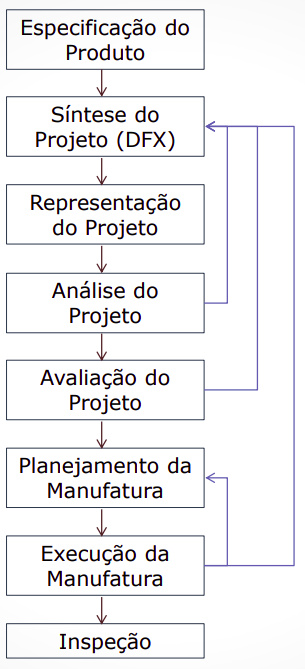
\includegraphics[width=0.3\textwidth]{product_development.png}
\end{figure}

\begin{description}
    \item[Especificação do Produto] é obtida a partir das exigências do consumidor.
    \item[Síntese do Projeto] é o processo de conversão das especificações em um conceito de produto.
\end{description}

Com o conceito do produto, inicia-se o detalhamento geométrico. No caso do \emph{projeto para manufatura} é importante lembrar das regras de projeto, isso é, nem todas as operações são igualmente fáceis de se realizar.

\subsection*{Análise de Engenharia}

\begin{description}
    \item[Montagem] Análise cinemática (funcionamento do produto com partes em movimento)
    \item[Peças individuais] Propriedades de tensão e temperaturas em condições operacionais
    \item[Ferramentas] Elementos finitos, simulações cinemáticas
\end{description}
Também é possível a utilização de prototipagem rápida para realizar a análise de engenharia.

Assim é possível realizar a avaliação do projeto, com várias alternativas com diferentes custos e funções, sendo possível combinar as alternativas para gerar diferentes soluções.

\subsection*{Planejamento da Manufatura}

Primeiro questionamento a ser respondido é relativo à terceirização do produto.

Caso seja manufaturado internamente, deve-se estabelecer o plano de processo para cada componente, ou seja, a sequência detalhada de operações contendo máquinas, ferramentas, operadores, parâmetros, etc.

Em relação ao processo, deve-se estabelecer uma programação mestre (MPS).

\subsubsection*{Lean Manufacturing}

Manufatura enxuta, foco na eficiência da produção. Equipamentos automatizados.

\subsection*{Inspeção}

Tanto no caso manual ou automática, o desenvolvimento de fixações e ferramentas específicas pode ser necessário. Para medir a qualidade de um produto, se faz necessário máquinas e fixações mais precisas do que o mesmo.

\section*{CAM}

\emph{Computer-Aided Manufacturing}, parte do CIM (\emph{Computer Integrated Manufacturing}). CAM representa o uso efetivo de computadores na manufatura, seja diretamente através do controle e monitoramento de processos (CNC, robótica, etc) ou indiretamente através do suporte às operações (planejamento e projeto de layout, scheduling, MRP, etc), vide figura abaixo.
 \begin{figure}[H]
    \centering
    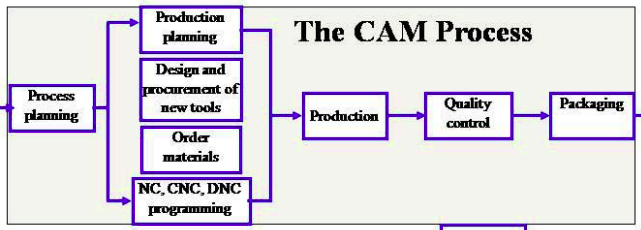
\includegraphics[width=0.8\textwidth]{cam_process.png}
\end{figure}

\section*{CAD e Manufatura}

\subsection*{O Papel do Computador no Projeto}

\begin{description}
    \item[Definição do problema] Computador pode não ser de grande auxílio para desenhar o produto frente especificações, mas é bastante efetivo em, após o projeto, sugerir projetos existentes e peças padronizadas ou processos de manufatura.
    \item[Modelagem geométrica] Descreve matematicamente a geometria de um objeto para representá-lo. Normalmente é feito através de um simplificação do objeto a suas características essenciais. Com o modelo é possível visualizar o objeto e animá-lo, possibilitando a detecção de problemas.
    \item[Análise de engenharia] Normalmente é empregada para otimizar um dado produto, normalmente em um estágio mais tardio do projeto pois requerem informações mais precisas. Bastante comum os softwares de elementos finitos.
    \item[Desenho automático] Fornecer informação do projeto para planejamento do processo, programação dos equipamentos. Dimensionamento automático é possível, além do fornecimento das vistas e cortes.
\end{description}

\subsection*{Construção de Elementos Geométricos no CAD}

Elementos geométricos são construídos a partir de elementos geométricos básicos.

\begin{description}
    \item[Cônicas] Parábolas, hipérboles e elipses. Podem ser sempre definidas a partir de 5 pontos (sem distinção da forma?).
    \item[Curvas e superfícies] Podem ser descritas a partir de pontos e uma expressão matemática que os interpole (e.g. Bézier, B-spline). Outra alternativa é a descrição através de \emph{patches} (\emph{blending}).
\end{description}

\emph{Wireframes}, que só contém pontos e arestas, possibilitam múltiplas interpretações pois não indicam quais são as arestas conectadas.

\subsection*{Modelagem e Base de Dados no CAD}

A base de dados do CAD contém elementos gráficos básicos (pontos, linhas, curvas) e elementos que definem a geometria e topologia do objeto. Topologia é a rede na qual os elementos geométricos são interconectados (aresta, vértice, face). Geometria mostra os itens que auxiliam a completar a descrição da forma (ponto, curva, superfície).

\subsubsection*{Representação CSG}

\emph{Constructive Solid Geometry} é uma representação através de uma árvore binária, em que os nós são operações de movimentos rígidos ou booleanas (união, interseção e diferença), e os nós terminais (folhas) são primitivas (sólidos básicos) ou movimentos rígidos. É importante que a operação de interseção seja alterada para não considerar partes de volume zero, como faces ou arestas pendentes.

Para representar os objetos, CSG utiliza \emph{half-spaces}, que são corpos fechados em uma só superfície (planos, cones, cilindros, esferas), dividindo o espaço, ou seja, pode representar um cubo através de 6 \emph{half-spaces} planos e um cilindro finito através de um \emph{half-space} cilíndrico (que é infinito) e dois \emph{half-spaces} planos paralelos e perpendiculares ao eixo de rotação do cilindro.

Vantagens:
\begin{itemize}
    \item Concisa
    \item Garante que os objetos são válidos
    \item Conversão para B-rep é confiável
\end{itemize}

\subsubsection*{B-rep (\emph{Boundary Representation})}

Representa um sólido através de \emph{patches}, faces interligadas representadas por arestas (que são formadas por vértices), que formam um subconjunto finito. Desta forma, B-rep representa a topologia de forma explícita. Apesar de não possuir ambiguidade, possui redundância, pois é possível "alcançar" componentes da representação de diferentes formas (\emph{e.g.}, um vértice pode vir da interseção de faces ou de arestas). Por conta disso, possui uma base dados maior do que CSG e, por consequência, demora mais para checar consistência.

A modificação da topologia de um sólido deve obedecer a fórmula de \textbf{Euler-Poincaré} \[
    F - E + V - H = 2 \cdot (B-G)
\], onde
\begin{itemize}
    \item $F$ é o número de faces
    \item $E$ é o número de arestas
    \item $V$ é o número de vértices
    \item $H$ é o número de furos
    \item $B$ é o número de sólidos quaisquer
    \item $G$ é o número de anéis
\end{itemize}

Operações booleanas são muito mais lentas no B-rep.

Vantagens:
\begin{itemize}
    \item Informações mais completas
    \item É mais fáceis para "desenhar"
\end{itemize}

\subsubsection*{Features}

\begin{definition}
    (Feature) Regiões ou volumes em peças industriais, que são importantes para o projeto, planejamento do processo e outras atividades.
\end{definition}

Exemplos comuns: furo (\emph{hole}), \emph{pocket}, \emph{shoulder}.

Features são muito úteis para a tomada de decisões de manufatura, por exemplo, quando sabemos que existe um furo na peça, podemos de prontidão determinar que pode ser feito por uma operação de furação utilizando uma peça rotacional. Portanto, auxilia na comunicação do sólido para o CAPP. Além disso, comunicam com maior facilidade com o projetista por trazerem informações funcionais e tecnológicas.

Pode-se representar a peça diretamente através de features, utilizando-as como "tijolos" do processo de design do produto.

\subsubsection*{Lista de Materiais (\emph{BOM})}

Estrutura de dados do produto que possui as informações dos componentes do produto final, suas quantidades e suas relações de forma hierárquica.

Tipos:
\begin{description}
    \item[Resumida] Lista única com a quantidade total de cada material, não indicam quando as peças devem ser encomendadas pois não deixa explícita a ordem de montagem.
    \item[Tabulada] As peças são repetidas para cada subconjunto, separando cada subconjunto em uma lista separada para evitar uma lista muito extensa.
\end{description}

\subsection*{Interfaces Padronizadas para CAD/CAD/CAM}

Visam reduzir os custos de comunicar diferentes softwares utilizados dentro do processo de manufatura de um produto (planejamento do processo, \emph{scheduling}, manufatura, controle de qualidade, etc. CAx). Geralmente os softwares armazenam as informações do produto em um formato proprietário, o que dificulta a comunicação. Uma interface neutra comum pode facilitar tanto a troca de informações entre softwares de diferentes etapas do processo como de um mesmo processo. Naturalmente, várias exigências existem e esse não é um desafio fácil.

\subsubsection*{IGES (\emph{Initial Graphic Exchange Specification})}

Objetiva a troca entre sistemas CAD. Tenta representar desenhos técnicos, \emph{wireframe}, superfícies e sólidos, modelos de elementos finitos, etc. Suporta várias entidades básicas e curvas.

\subsubsection*{STEP (\emph{Standard for External Representation of Product Data})}

Esforço internacional para representar todas as informações do ciclo de vida de um produto. Possui vários módulos internos para representar as informações das diferentes etapas do ciclo de vida. É normatizado pela ISO.

Possui métodos e princípios em 5 categorias:
\begin{description}
    \item[Método de descrição] Através da linguagem \emph{Express}, descreve o modelo do produto.
    \item[Método de implementação] Definem as interfaces para transferir os dados de \emph{Express} para outros aplicativos.
    \item[Metodologia de ensaio para conformidade e estrutura] Visa testar a conformidade de implementações de qualquer Protocolo de Aplicação (AP) ou suas combinações.
    \item[Recurso para a integração da informação] Modelos de dados genéricos da norma STEP, que auxiliam na integração das APs.
	\begin{description}
	    \item[Recursos para integração genérica] definem modelos que não dependem da aplicação, \emph{e.g.}, geometria e topologia, apresentação visual.
	    \item[Recursos para integração da aplicação] especificam extensões para os arquivos genéricos, com um pouco mais de contexto.
	\end{description}
    \item[Protocolos de Aplicação] São grupos de entidades únicas escolhidos para finalidades \textbf{específicas}, \emph{e.g.}, indústria automobilística, naval, desenho e planejamento de chapas.
\end{description}

\subsection*{Exigências de um Modelo de Produto}

Durante a fase de projeto estabelece-se 70\% ou mais do custo associado ao produto ao longo de sua vida.

Durante cada etapa do desenvolvimento, as etapas seguintes devem ser levadas em consideração, por exemplo, o projetista deve pensar em como a peça será fabricada durante o design. Isso pois mudanças no produto aumentam drasticamente com o evoluir do processo.

\emph{Engenharia simultânea} visa integrar a manufatura e demais etapas do ciclo de vida de um produto na etapa de projeto, contrariando a engenharia sequencial tradicional. Dessa forma, evitam-se correções e retrabalho. Em geral, o engenheiro de manufatura define regras a serem seguidas pelo projetista para garantir a manufaturabilidade do produto.

Regras básicas do \emph{Projeto para Manufatura - DFM}:
\begin{itemize}
\item usar peças padronizadas sempre que possível;
\item tirar vantagem da forma geométrica do material a ser trabalhado para projetar as peças;
\item usar projetos anteriores sempre que possível;
\item minimizar a quantidade de usinagem sempre que possível;
\item durante o projeto da forma geométrica, considerar a facilidade de manuseio de material, fixação, usinagem e montagem;
\item Utilizar tolerâncias e acabamentos adequados para o processo de manufatura e montagem;
\item considerar os princípios cinemáticos durante os passos iniciais do projeto.
\end{itemize}

Estágios importantes no \emph{Projeto para Montagem}:
\begin{itemize}
    \item Alimentação das peças
	\item Orientação das peças
	    \item Apresentação das peças
		\item Custo do sistema de manuseio
\end{itemize}

Regras para o \emph{Projeto para a Manufatura e Montagem - DFMA}:
\begin{enumerate}
    \item Minimizar o número de peças;
    \item Minimizar as superfícies montadas;
    \item Projetar para montagem de cima para baixo: gravidade;
    \item Melhorar acesso para montagem;
    \item Maximizar a concordância entre as peças: ranhuras adequadas e superfícies guia;
    \item Maximizar a simetria das peças: mais fáceis de orientar;
    \item Otimizar o manuseio das peças: superfícies adequadas para aperto mecânico + obstáculos para evitar emaranhamento;
    \item Evitar fixadores separados: snap-fit.
    \item Fornecer peças com características de auto-fixação: dentes ou projeções para manter a orientação até a montagem final.
    \item Focalizar em projeto modular: peças com função comum $\implies$ peça ou módulo padrão; peças intercambiáveis $\implies$ interface padrão.
\end{enumerate}

Pode-se estimar a eficiência do projeto pela equação \[
EM = \frac{3\times NM}{TM}
\], ondoe $NM$ é o número mínimo teórico de peças e $TM$ é o tempo total de montagem manual.

\subsection*{Controle de Variantes de Projeto de Produtos}

Para reduzir os custos e reduzir o \emph{lead time}, é muito útil manter uma estrutura modular dos produtos. Isso também aumenta a agilidade de responder às mudanças de mercado. Também reduz os estoques, pois reduz a quantidade de "linhas" para uma grande quantidade de produtos.

\begin{description}
    \item[Slot] aceita diferentes versões de um mesmo produto, e.g., rádio do carro.
    \item[Bus] aceita componentes completamente diferentes, e.g., porta USB.
    \item[Sectional] possui interfaces idênticas e os componentes se conectam entre si.
\end{description}

\section*{Prototipagem Rápida}

Para gerar o modelo inicial de um novo projeto e poder realizar testes preliminares, hoje sabe-se que é mais vantajoso adotar métodos rápidos ao invés de envolver operadores experientes em uma oficina. Manufatura aditiva = impressão 3D.

\begin{description}
    \item[Estereolitografia] tanque com polímero líquido fotosensitivo, seguido de um forno para dar resistência.
    \item[Sinterização Seletiva a Laser (SLS)] similar ao anterior, mas utiliza o laser para fundir ou sinterizar. Custo menor e melhores propriedades mecânicas, mas com menor tolerâncias.
    \item[Modelagem por Deposição por Fundição (FDM)] deposita um fio fino de plástico ou cera formando as camadas. Processo rápido e materiais mais baratos.
    \item[Manufatura de Objetos Laminados (LOM)] cada "fatia" do material é cortada e unida por adesivo ao objeto. Muito mais rápido que os outros processos.
    \item[\emph{Laser Metal Deposition}] pó metálico é depositado em uma poça fundida por um laser no objeto, similar à FDM, mas para metal.
    \item[Two-Photon Polymerization] laser para formar estruturas microscópicas.
    \item[Binder Jetting (BJ)] apesar da estrutura similar ao SLS, ao invés de laser o cabeçote deposita um ligante ao pó.
\end{description}

\section*{Precisão e Erros de Usinagem}

Muito além dos parâmetros geométricos. Diferença entre os parâmetros reais e os parâmetros definidos no projeto é a qualidade da peça. A proximidade dos parâmetros macro-geométricos é chamada \emph{precisão de usinagem}; a proximidade entre os parâmetros micro-geométricos é chamada \emph{qualidade da superfície}.

Precisão de usinagem de superfície pode ser relativa às dimensões (e.g., diâmetros de superfícies cilíndricas) ou as formas (e.g., planicidade) de superfícies. Precisão de usinagem de posições relativas refere às dimensões entre superfícies ou relações (e.g., paralelismo).

Métodos para obter precisão dimensional exigida:
\begin{description}
    \item[Tentativas] baixa eficiência, baixo custo de setup.
    \item[Dimensão automática] uso de ferramentas de dimensão e forma fixa, máquinas presetadas, dispositivos guias, comando numérico.
\end{description}

Fatores que causam erros de usinagem:
\begin{itemize}
    \item Posicionamento da ferramenta em relação à máquina e da peça em relação à máquina $\implies$ precisão relativa entre as ferramentas e a peça.
	\item Desgaste das máquinas e ferramentas
	    \item Imprecisão das ferramentas
		\item Deformação por forças externas.
\end{itemize}

\end{document}
